% !TeX root = Tutorial_13_Two-phase_flow.tex

\documentclass[a4paper, 14pt, twoside]{article}
\usepackage[14pt]{extsizes}
\usepackage[english,russian]{babel}
\usepackage[utf8]{inputenc}
\usepackage{amsfonts, amsmath, amssymb,amsthm, graphics,latexsym}
\usepackage{color}
\usepackage{wasysym}
\usepackage{misccorr}
\usepackage{mathrsfs}
\usepackage[active]{srcltx}
\usepackage{amsthm,fullpage}
\usepackage{fullpage}
\usepackage{multicol}
\usepackage[pdftex]{graphicx}
\usepackage[square, numbers]{natbib}
%\usepackage{fancyhrd}
%\usepackage{morefloats}
\usepackage{caption}
\usepackage{xcolor}
\usepackage{ifthen}
\usepackage{verbatim}
\usepackage{makeidx}
\usepackage{enumerate}
\usepackage{float}
\usepackage{graphicx,fancybox}
\usepackage{bm}
\usepackage{pdfcomment}
%\usepackage{indentfirst}
% \usepackage{commath}

\usepackage{hyperref} % For \url command

\usepackage{mathtools} % for def over equal sign command

\usepackage[makeroom,thicklines]{cancel} % For commands to cross-out math symbols. See http://tex.stackexchange.com/questions/75525/how-to-write-crossed-out-math-in-latex

\usepackage[left=3cm,right=2cm,
    top=3cm,bottom=3cm,bindingoffset=0cm]{geometry}
    
\usepackage{empheq} % for empheq environment
\usepackage{listingFreeFem}
\usepackage{appendix}

\lstset{
	columns=fullflexible,
	frame=shadowbox,
	numbers=left,
	numberstyle=\color{gray},
	breaklines=true,
	postbreak=\mbox{\textcolor{red}{$\hookrightarrow$}\space},
}



    
%\fontsize{14}{16pt}\selectfont \sloppy \allowdisplaybreaks
%%\renewcommand{\baselinestretch}{1.5}
%\sloppy


%%%%%%%%%%%%%%%%%% COLORS %%%%%%%%%%%%%%%%%%%%%%%%%%%%%
\renewcommand{\CancelColor}{\color{red}} % Color for canceling terms in expression

% Command for text highlighting
% Usegae:
%       \highlight{text}{color}
\newcommand{\highlight}[2]{
    \textbf{\color{#2}#1}}  % 

\newcommand{\todo}[1]{\textbf{\color{red}#1}}

%%%%%%%%%%%%%%%%%% MATH OPERATORS %%%%%%%%%%%%%%%%%%%%%%%%%%%%%
\DeclareMathOperator\dv{div} % divegence
\DeclareMathOperator\id{I}   % identity matrix
\DeclareMathOperator\tr{tr}  % trace operator
\DeclareMathOperator{\E}{E}  % Large strain tensor
\DeclareMathOperator{\const}{const} % const value 
\DeclareMathOperator{\rank}{rk}
%%%%%%%%%%%%%%%%%% BOLD SYMBOLS %%%%%%%%%%%%%%%%%%%%%%%%%%%%%
\newcommand{\bX}{\mathbf{X}}  % bold X
\newcommand{\bv}{\bm{v}}  % bold v
\newcommand{\bu}{\mathbf{u}}  % bold u
\newcommand{\bw}{\mathbf{w}}  % bold w
\newcommand{\bq}{\mathbf{q}}  % bold q
\newcommand{\bx}{\mathbf{x}}  % bold x
\newcommand{\be}{\mathbf{e}}  % bold e
\newcommand{\bs}{\mathbf{s}}  % bold s
\newcommand{\bn}{\mathbf{n}}  % bold n
\newcommand{\bp}{\mathbf{p}}  % bold p
\newcommand{\bff}{\mathbf{f}}  % bold f
\newcommand{\bc}{\mathbf{c}}  % bold c
\newcommand{\bbf}{\mathbf{f}}  % bold f
\newcommand{\bt}{\mathbf{t}} % bold T

\newcommand{\bD}{\mathbf{D}}  % bold D
\newcommand{\bP}{\mathbf{P}}  % bold P
\newcommand{\bcu}{\mathbf{U}} % bold U
\newcommand{\bct}{\mathbf{T}} % bold T

\newcommand{\bpsi}{\boldsymbol{\psi}} % bold psi
\newcommand{\bsigma}{\boldsymbol{\sigma}} % bold sigma
\newcommand{\btau}{\bm{\tau}} % bold tau
%%%%%%%%%%%%%%%%%% CALLIGRAPHIC SYMBOLS %%%%%%%%%%%%%%%%%%%%%%%%%%%%%
\newcommand{\epss}{{\cal E}}
\newcommand{\cL}{{\cal L}}
\newcommand{\cT}{{\cal T}}
\newcommand{\cQ}{{\cal Q}}

%%%%%%%%%%%%%%%%%% DIFFERENTIAL OPERATORS %%%%%%%%%%%%%%%%%%%%%%%%%%%%%
\newcommand{\pd}[2]{ % partial first derivative
   \dfrac{\partial #1}{\partial #2}
} 
\newcommand{\opd}[2]{ % ordinary first derivative
    \dfrac{\mathrm{d} #1}{\mathrm{d} #2}
}
\newcommand{\pddB}[2]{ % partial first derivative with function bordered by braces
    \dfrac{\partial }{\partial #2}\Bigl(#1\Bigr)
} 
\newcommand{\pdd}[3]{ % partial second mixed derivative
    \dfrac{\partial^2 #1}{\partial #2 \partial #3}
}

\newcommand{\pddfirst}[2]{ % partial second derivative with respect to one variable
    \frac{\partial^2 #1}{\partial {#2}^2}
}

%%%%%%%%%%%%%%%%%% NEW COMMANDS %%%%%%%%%%%%%%%%%%%%%%%%%%%%%
\newcommand\myeq{\stackrel{\mathclap{\footnotesize \mbox{def}}}{=}}

%%%%%%%%%%%%%%%%%% RENEW COMMANDS %%%%%%%%%%%%%%%%%%%%%%%%%%%%%
\renewcommand{\leq}{\leqslant} % Beautiful <=
\renewcommand{\geq}{\geqslant} % Beautiful >=

%%%%%%%%%%%%%%%%%% THEOREM STYLES %%%%%%%%%%%%%%%%%%%%%%%%%%%%%
\theoremstyle{definition}
\newtheorem{Lemma1}{Лемма}
\theoremstyle{definition}
\newtheorem{Problem}{Задача}
\newtheorem{Definition}{Определение}

\theoremstyle{remark}
\newtheorem*{Solution}{РЕШЕНИЕ}
\newtheorem*{Tip}{ПОДСКАЗКА}

%%%%%%%%%%%%%%%%%% PATHS TO FOLDERS WITH IMAGES %%%%%%%%%%%%%%%%%%%%%%%%%%%%%
\graphicspath{{img/}}

%%%%%%%%%%%%%%%%%% OTHER CUSTOMIZATIONS %%%%%%%%%%%%%%%%%%%%%%%%%%%%%
\everymath{\displaystyle} % Make all maths looks good

\DeclareMathOperator{\diver}{div}
\DeclareMathOperator\arctanh{arctanh}


%\textheight 240mm
%\textwidth 16cm
%\topmargin -15mm %было-15mm
%\multlinegap=0pt
\author{Калинин С.А., Кузнецов В.А., Стамлер К.В.}

%\title{Семинары по <<Введению в МСС>>}




\title{Задача моделирования дфухфазной 2D фильтрации при наличии добывающей и нагнетательной скважины}

\begin{document}
\maketitle



\section{Краткое описание решаемой задачи}

Требуется численно решить проблему двухфазной фильтрации воды и нефти в двумерной области при 
наличии добывающих и нагнетательных скважин. Для этого сначала записывается математическая 
формулировка задачи в дифференциальной и слабой постановке,
а далее используется пакет с открытым исходным кодом "FreeFem++". В качестве численного
метода во FreeFem++ используется метод конечных элементов.\\
В отличие от рассмотренной в учебном курсе упрощенной задачи Баклея-Леверетта, где скорость по
все расчетной области принималась постоянной, в данной работе учитывается 
наличие различного градиента давления в различных точках области. Кроме того, в качестве
функций источника необходимо использовать точечные источники (соответствуют нагнетательным
вертикальным скважинам) и стоки (добывающие вертикальные скважины). Использование точечных 
источников предполагает обращение к отдельным узлам расчетной сетки, что осложняет численную
реализацию решения задачи.

\section{Основные соотношения}

\subsection{Обозначения}

Здесь и далее жирными буквами обозначены векторные или тензорные величины. Ниже приведен список
используемых переменных и указана их размерность в СИ\\
$S_w$~---~насыщенность водой [безразм.];\\
$\phi$~---~пористость [безразм.];\\
$\rho_w$~---~плотность воды [$\text{кг}/\text{м}^3$];\\
$\bm{v}_{rw}$~---~относительная скорость фильтрации воды в присутствии нефти;\\
$\bm{v}_{ro}$~---~относительная скорость фильтрации нефти в присутствии воды;\\
$q_w$~---~удельный (на мощность пласта, т.е. $[\text{м}^2/\text{с}]$) расход или поток воды;\\
$q_o$~---~удельный (на мощность пласта, т.е. $[\text{м}^2/\text{с}]$) расход или поток нефти;\\ 
$q_t$~---~удельный (на мощность пласта, т.е. $[\text{м}^2/\text{с}]$) полный расход флюида;\\ 
$K$~---~абсолютная проницаемость (в общем случае тензор) [$\text{м}^2$];\\
$k_{rw}$~---~относительная фазовая проницаемость по воде [безразм.];\\
$k_{ro}$~---~относительная фазовая проницаемость по нефти [безразм.];\\
$p_w$~---~давление в водной фазе [Па];\\
$p_o$~---~давление в нефтяной фазе [Па];\\
$\mu_w$~---~вязкость воды [Па*с];\\
$\mu_o$~---~вязкость нефти [Па*с];\\
$\nabla$~---~оператор градиента;\\
$\bm{n}$~---~вектор внешней нормали;\\
$\overline{\bm{q}}_\alpha$~---~заданный поток на границе, где $\alpha \in \{inj,prod\}$;\\
$R_\Omega$~---~невязка дифференциального уравнения внутри расчетной области;\\
$R_\Gamma$~---~невязка для граничного условия по границе расчетной области;\\
$\xi$~---~весовая функция для расчета давления, заданная во внутренних точках области;\\
$\overline{\xi}$~---~весовая функция для расчета давления на границе расчетной области;

\subsection{Дифференциальная постановка}
Уравнения двухфазного течения в породе включают в себя уравнения для переноса воды и нефти
\begin{equation}\label{eq:egor_common_equation_multiphase_rho}
\begin{split}
	\pd{(S_w \phi \rho_w)}{t} + \dv(\rho_w \bm{v}_{rw})    &= - \rho^{st}_w q_w, \quad \bm{v}_{rw}=-\frac{K k_{rw}}{\mu_w}\nabla p_w,\\
	\pd{(S_o \phi \rho_o)}{t} + \dv(\rho_o \bm{v}_{ro})  &= - \rho^{st}_o q_o, \quad \bm{v}_{ro}=-\frac{K k_{ro}}{\mu_o}\nabla p_o.
\end{split}
\end{equation}

$$
\rho_\alpha(p_\alpha) = \frac{\rho^{st}_\alpha}{B_\alpha}, \quad \alpha = w,o,
$$
где $\rho^{st}_\alpha,$~$B_\alpha$~---~плотности фильтрующихся жидкостей при некоторых стандартных (референсных) условиях и  коэффициенты объемного расширения соответственно. 
Тогда сжимаемости воды и нефти примут вид 
\begin{equation}\label{eq:sibin_c_alpha}
c_\alpha = \frac{1}{\rho_\alpha} \pd{\rho_\alpha}{p_\alpha} = B_\alpha \pd{(1 / B_\alpha)}{p_\alpha}, \quad \alpha = w,o.
\end{equation}

Введем масштабированную насыщенность
\begin{equation}\label{eq:star:mod:Sw}
 \overline {S}_w= \frac{S_w-S_w^{cr}}{1-S_w^{cr}-S_o^{cr}},
\end{equation}
где $S_w^{cr}$ --- критическая водонасыщенность, при которой перестает течь вода, $S_o^{cr}$ --- критическая нефтенасыщенность, при которой перестает течь нефть. Тогда относительные фазовые проницаемости можно записать в следующем виде:
\begin{equation}\label{eq:star:mod:RelatPerm}
	k_{rw}= \begin{cases}
	0, \quad \text{при}\quad \overline {S}_w \leq 0,\\
	k_{rw}^0 (\overline {S}_w)^{n_w}, \,\text{при}\,0<\overline {S}_w <1, \\
	k_{rw}^0, \text{при}\quad \overline {S}_w \geq 1.
   \end{cases}
   k_{ro}=\begin{cases}
	k_{ro}^0, \quad \text{при}\quad \overline {S}_w \leq 0, \\
	k_{ro}^0 (1-\overline {S}_w)^{n_o}, \, \text{при}\,0<\overline {S}_w<1 , \\
   0, \quad \text{если}\quad \overline {S}_w \geq 1.\\
   \end{cases}
\end{equation}

\begin{figure}[H]
	\centering
	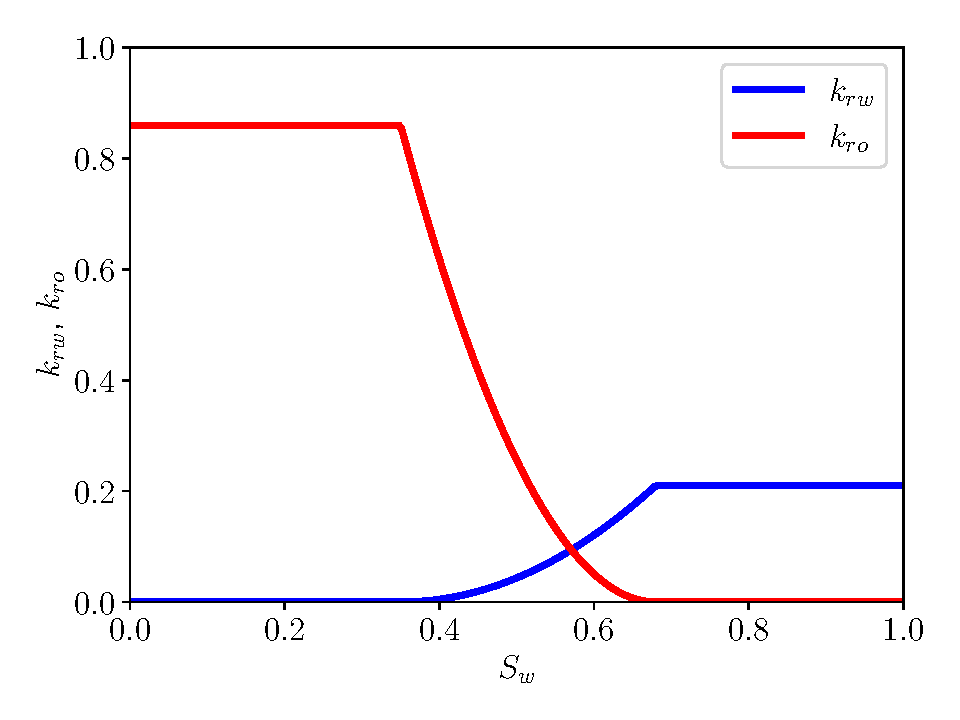
\includegraphics[width=0.7\linewidth]{img/RPP_Corey}
	\caption{Кривые ОФП по модели Кори}
	\label{fig:RPP_Corey}
\end{figure}

\subsubsection{Упрощающие предположения}
Будем считать, что коэффициеты объемного расширения постоянны в рассматриваемом диапазоне давлений и равны $B_\alpha = 1$, $\alpha = w,o$. Также пренебрежем влиянием капилярных сил:
\begin{equation}\label{eq:common_eq_capillar}
	p_c(S_w) = p_o - p_w = 0,
\end{equation}
что влечет равенство давлений в фазах.
Для насыщенностей фаз имеется соотношение
\begin{equation}\label{eq:So_Sw_1}
	S_o + S_w = 1.
\end{equation}
Предположим, что поровое пространство слабосжимаемое. Тогда
\begin{equation}\label{eq:compress_phi}
	c_r = \frac{1}{\phi} \pd{\phi}{p}, \quad p = p_w=p_o,
\end{equation}
при этом сама пористость приближенно считается постоянной $\phi=\phi_0$.

\subsubsection{Формулировка в переменных $p$---$S_w$}

Складывая уравнения с учетом упрощающих предположений, получим

\begin{equation}
    c_t\phi \pd{p}{t}
    + \dv\, \left( -\left(\frac{K k_{rw}}{\mu_w } +
     \frac{K k_{ro}}{\mu_o}\right)\nabla p \right) = q_w + q_o,
\end{equation}
$c_t= c_r + c_w  S_w + c_o (1-S_w)$ --- полная сжимаемость системы, включающая сжимаемости пор $c_r$ воды $c_w$ и нефти $c_o$.
Уравнение на насыщенность воды запишется в виде
\begin{equation}\label{eq:star_common_equation_multiphase_satur}
	  \phi \pd{S_w}{t} + S_w\phi\left(c_r + c_w \right)\pd{p}{t} + \dv\, \left( -\frac{K k_{rw}}{\mu_w}\nabla p \right) = 
	  q_w.
\end{equation}

Заметим, что если ввести обозначения
\begin{equation}
    \bq_w = -K\frac{k_{rw}(S_w)}{\mu_w}\nabla p = -K \lambda_w(S_w) \nabla p,
\end{equation}
\begin{equation}
	\bq_o = -K\frac{k_{ro}(S_w)}{\mu_o}\nabla p = -K \lambda_o(S_w) \nabla p,
\end{equation}
то полный фильтрационный поток жидкости выражается в виде
\begin{equation}
    \bq_t = \bq_w + \bq_o = -K (\lambda_w(S_w) + \lambda_o(S_w)) \nabla p = -K (\lambda_t(S_w)) \nabla p,
\end{equation}
а фильтрационный поток воды можно записать как 
\begin{equation}
    \bq_w = f_w \bq_t, \quad f_w  = \dfrac{\lambda_w(S_w)}{\lambda_t(S_w)},
\end{equation}
где $f_w$ --- функция Баклея~---~Леверетта.

В этих терминах основные уравнения записываются в следующем виде:
\begin{equation}
    c_t\phi \pd{p}{t}
    + \dv\, \left( \bq_t \right) = q_w + q_o, \quad \bm{q}_{t} = - K \lambda_t \nabla p,
\end{equation}

\begin{equation}\label{eq:satur}
	\phi \pd{S_w}{t} + S_w\phi\left(c_r + c_w \right)\pd{p}{t} + \dv\, \left( f_w \bq_t \right) = 
	q_w.
\end{equation}
В общем случае также необходимо решить уравнение на эволюцию пористости
\begin{equation}\label{eq:porosity_evolution}
	\pd{\phi}{t} = \pd{\phi}{p} \pd{p}{t}  = c_r \phi \pd{p}{t}.
\end{equation}

\subsubsection{Задача Баклея~---~Леверетта}

Рассмотрим классическую задачу Баклея~---~Леверетта о вытеснении нефти водой для пятиточечного
шаблона заводнения. 
Предположим, что нам задана прямоугольная область $\Omega$ (рисунок~\ref{fig:ProblemInitBoundary}), 
внутри которой выполняются уравнения двухфазной фильтрации. 
\begin{figure}[H]
	\centering
	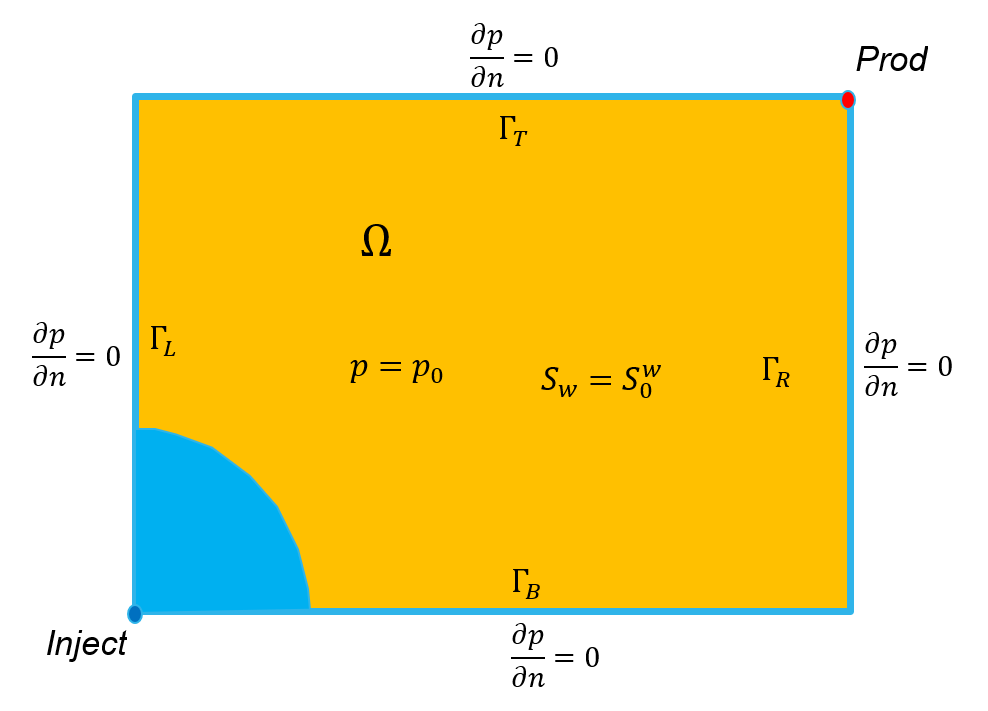
\includegraphics[width=1\linewidth]{img/ProblemInitBoundary}
	\caption{Постановка задачи Баклея --- Леверетта для пятиточечного шаблона заводнения}
	\label{fig:ProblemInitBoundary}
\end{figure}

В силу симметрии задачи поток через все границы отсутствует, поэтому достаточно записать
\begin{equation}
	\Gamma_L, \Gamma_R, \Gamma_T, \Gamma_B: \quad \bq_t \cdot \bn = 0,
\end{equation}

Через левый нижний узел прямоугольной области производится закачка воды с заданным 
расходом и насыщенностью:
\begin{equation}\label{eq:GammaL}
	\Gamma_{Inj}: \bm{q}_{t} = \overline{\bm{q}}_{inj}, \quad S_w = S_w^{inj}.
\end{equation}
Через верхний правый узел происходит добыча флюида
\begin{equation}\label{eq:GammaR}
	\Gamma_{Prod}: \bm{q}_{t} = \overline{\bm{q}}_{prod}.
\end{equation}


\textbf{Замечание.} Уравнение на насыщенность гиперболического типа, поэтому граничное 
условие ставится только на той границе, где характиристики уравнения входят в область.

В качестве начальных данных задаются следующие величины:
\begin{equation}\label{eq:init_cond}
	\Omega: \quad S_w\left|_{t=0} = S_w^0\right., \quad p\left|_{t=0} = p_0\right.  \quad \phi\left|_{t=0} = \phi_0\right..
\end{equation}



\subsection{Слабая постановка}


\subsubsection{Уравнение фильтрации}
Для получения слабой формулировки воспользуемся общим алгоритмом метода взвешенных невязок 
(\cite{Zenkevich_1986} стр.59 ур.(2.41)). В общем случае полагается, что системы весовых
функций для области $\Omega$ и границы $\Gamma$ отличаются, тогда
 \begin{equation}
	\int\limits_\Omega \xi R_\Omega \,d\Omega + \int\limits_\Gamma \overline{\xi}R_\Gamma \,d\Gamma = 0
 \end{equation} 
В качестве тестовой функции для давления выберем $\xi$, при этом 
\begin{equation}
	\xi\left|_{\Gamma_L}\right. = 0.
\end{equation}

Тогда 

\begin{multline}
	\displaystyle 0=\int\limits_\Omega c_t\phi \pd{p}{t}\, \xi \,dx dy 
	 + \int\limits_\Omega \dv{\bq_t}\, \xi \,dx dy= \\ 
	 \int\limits_\Omega c_t\phi \pd{p}{t}\, \xi \,dx dy 
	 + \int\limits_\Omega K \lambda_t \nabla p \cdot \nabla\xi \,dx dy \\
	 +\int\limits_{\Gamma_L} (\bq_t \cdot \bn) \xi \, ds
	 +\int\limits_{\Gamma_T\cup \Gamma_B} (\bq_t \cdot \bn) \xi \, ds
	 +\int\limits_{\Gamma_R} (\bq_t \cdot \bn) \xi \, ds= \\
	 \int\limits_\Omega c_t\phi \pd{p}{t}\, \xi \,dx dy 
	 + \int\limits_\Omega K \lambda_t \nabla p \cdot \nabla\xi \,dx dy -\int\limits_{\Gamma_L} q_{inj} \xi \, ds \\
\end{multline}

\subsubsection{Уравнение переноса водонасыщенности}

Если применить стандартный прием метода конечных элементов к исходному уравнению на водонасыщенность, то известно, что получится неустойчивая разностная схема. 
Поэтому к исходному уравнению на водонасыщенность добавим член с искусственной диффузией. С физической точки зрения данное слагаемое появляется из-за присуствия капилярных сил. В итоге получим 

\begin{equation}\label{eq:satur_diffusion}
	\phi \pd{S_w}{t} + S_w\phi\left(c_r + c_w \right)\pd{p}{t} + \dv\, \left( f_w \bq_t {- \color{blue}\varepsilon \nabla S_w} \right) = 
	q_w.
\end{equation}
На практике параметр $\varepsilon$ может иметь зависимость от размера сетки и/или от величины градиентов решения, зануляться в окрестности границ.

На границах без условия Дирихле нам потребуется задать граничное условие отсуствия диффизионного потока в виде
\begin{equation}\label{eq:GammaTBR_Sw_diffusion}
	\Gamma_T, \Gamma_B, \Gamma_R: \quad \nabla S_w \cdot \bn = 0.
\end{equation}

Для перехода к слабой постановке в качестве тестовой функции выберем $\psi$ для водонасыщенности, при этом 
\begin{equation}
	\psi\left|_{\Gamma_L}\right. = 0.
\end{equation}

Тогда 

\begin{multline}
	\displaystyle 0=\int\limits_\Omega  \left(\phi \pd{S_w}{t} + S_w\phi\left(c_r + c_w \right)\pd{p}{t} \right)\,\psi + \dv\, \left( f_w \bq_t - \varepsilon \nabla S_w \right)\, \psi \,dx dy = \\ 
	\left(\phi \pd{S_w}{t} + S_w\phi\left(c_r + c_w \right)\pd{p}{t} \right)\,\psi \,dx dy - \int\limits_\Omega  f_w \bq_t \cdot \nabla \psi + \int\limits_\Omega \varepsilon \nabla S_w \cdot \nabla \psi \,dx dy  \\
	+\int\limits_{\Gamma_L} \left(f_w \bq_t - \varepsilon \nabla S_w \right)\cdot \bn\, \psi \, ds
	+\int\limits_{\Gamma_T\cup \Gamma_B} \left(f_w \bq_t - \varepsilon \nabla S_w \right)\cdot \bn \, \psi \, ds \\
	+\int\limits_{\Gamma_R} f_w \bq_t \cdot \bn \,\psi \, ds
	-\int\limits_{\Gamma_R} \varepsilon \nabla S_w \cdot \bn\, \psi \, ds = \\
	\int\limits_\Omega \left(\phi \pd{S_w}{t} + S_w\phi\left(c_r + c_w \right)\pd{p}{t} \right)\,\psi -  f_w \bq_t \cdot \nabla \psi +  \varepsilon \nabla S_w \cdot \nabla \psi \,dx dy \\
	+\int\limits_{\Gamma_R} f_w \bq_t \cdot \bn \,\psi \, ds
\end{multline}

\subsubsection{Дискретизация по времени и нелинейности}

Пусть $f^{n}$ --- значение функции на шаге по времени $n$. $f^{n+1,k}$ --- значения функции на $(n+1)$ шаге по времени на $k$-й итерации. Тогда можно ввести следующую дискретизацию по времени и нелинейности:

\begin{equation}
	\pd{p}{t} \approx \dfrac{p^{n+1, k+1}-p^{n}}{\Delta t}, \quad \pd{S_w}{t} \approx \dfrac{S_w^{n+1, k+1}-S_w^{n}}{\Delta t}, \quad \pd{\phi}{t} \approx \dfrac{\phi^{n+1, k+1}-\phi^{n}}{\Delta t},
\end{equation}

\begin{equation}
	f_w(S_w^{n+1, k+1}) = f_w(S_w^{n+1, k}) + \pd{f_w}{S_w}\Bigl|_{S_w^{n+1, k}}\Bigr. \left( S_w^{n+1, k+1} - S_w^{n+1, k} \right) .
\end{equation}

В данных обозначениях можно линеаризовать уравнения на давление в виде

\begin{multline}
	 \int\limits_\Omega c_t (S_w^{n+1, k})\phi^{n+1, k} {\color{red}p^{n+1, k+1}}\, \xi \,dx dy 
	 + \Delta t \int\limits_\Omega K \lambda_t (S_w^{n+1, k}) \nabla {\color{red}p^{n+1, k+1} }\cdot \nabla\xi \,dx dy \\ -\int\limits_\Omega c_t (S_w^{n+1, k})\phi^{n+1, k} p^{n}\, \xi \,dx dy-\Delta t \int\limits_{\Gamma_L} q_{inj} \xi \, ds=0
\end{multline}

После этого расчитывается 
\begin{equation}
	\bq_t^{n+1, k+1} = -K\lambda_t (S_w^{n+1,k})\nabla {\color{red}p^{n+1, k+1} }.
\end{equation}
После этого решается уравнения на водонасыщенность

\begin{multline}
	\int\limits_\Omega \left(\phi^{n+1,k} {\color{blue}S_w^{n+1,k+1}} + {\color{blue}S_w^{n+1,k+1}}\phi^{n+1,k}\left(c_r + c_w \right)({\color{red}p^{n+1,k+1}} - p^n)  \right)\,\psi \,dx dy \\
	+ \Delta t\int\limits_\Omega -f_w ({\color{blue}S_w^{n+1,k+1}}) \bq_t^{n+1, k+1} \cdot \nabla \psi +  \varepsilon \nabla {\color{blue}S_w^{n+1,k+1}} \cdot \nabla \psi \,dx dy \\
	-\int\limits_\Omega \phi^{n+1,k} S_w^{n} \,\psi \,dx dy
	+\Delta t\int\limits_{\Gamma_R} f_w({\color{blue}S_w^{n+1,k+1}}) \bq_t^{n+1, k+1} \cdot \bn \,\psi \, ds = 0.
\end{multline}

Пористость обновляется из следующего соотношения:
\begin{equation}
	\phi^{n+1, k+1} = \phi^n + c_r \phi^{n+1, k} (p^{n+1, k+1} - p^n).
\end{equation}

\subsection{Точное решение }

Точное решение задачи Баклея~---~Леверетта в несжимаемом случае может быть найдено методом характеристик как (см.~\cite{Barenblatt_Entov_Ryzhik_1984} стр.~128, и \cite{Collins_1984} стр.~189)

\begin{equation}\label{exactSol_test}
	\begin{split}
		& f_w'(S_w) = \dfrac{x}{t} \dfrac{\phi}{q_{inj}}, \quad \text{если}\, S_w > S_f \text{ или } x < x_f, \\
		 & S_w=S_w^0, \quad \text{иначе} \\
	\end{split}
	\end{equation}
	где $x_f$ --- положение фронта в момент $t$ , $S_f$ --- водонасыщенность на фронте.
Решение представляет из себя волну разрежения, которая примыкает к ударной волне.

Водонасыщенность на фронте $S_f$ разрыва находится из условия равенства скорости характеристики и скорости ударной волны (Рис.~\ref{fig:FwCurveTangent}, волна разрежения <<догоняет>> ударную волну) как

\begin{equation}\label{eq:u_shock_ch}
	u_{ch} = \dfrac{q_{inj}}{\phi} \frac{\partial f_w}{\partial S_w}(S_f) = \dfrac{q_{inj}}{\phi} \dfrac{(f_w(S_f)-f(S_w^0))}{(S_f-S_w^0)} = u_{shock}
\end{equation}
или
\begin{equation}\label{eq:S_front_eq}
	(S_f-S_w^0)\cdot \frac{\partial f_w}{\partial S_w}(S_f)=f_w(S_f)-f(S_w^0).
\end{equation}
\begin{figure}[H]
	\centering
	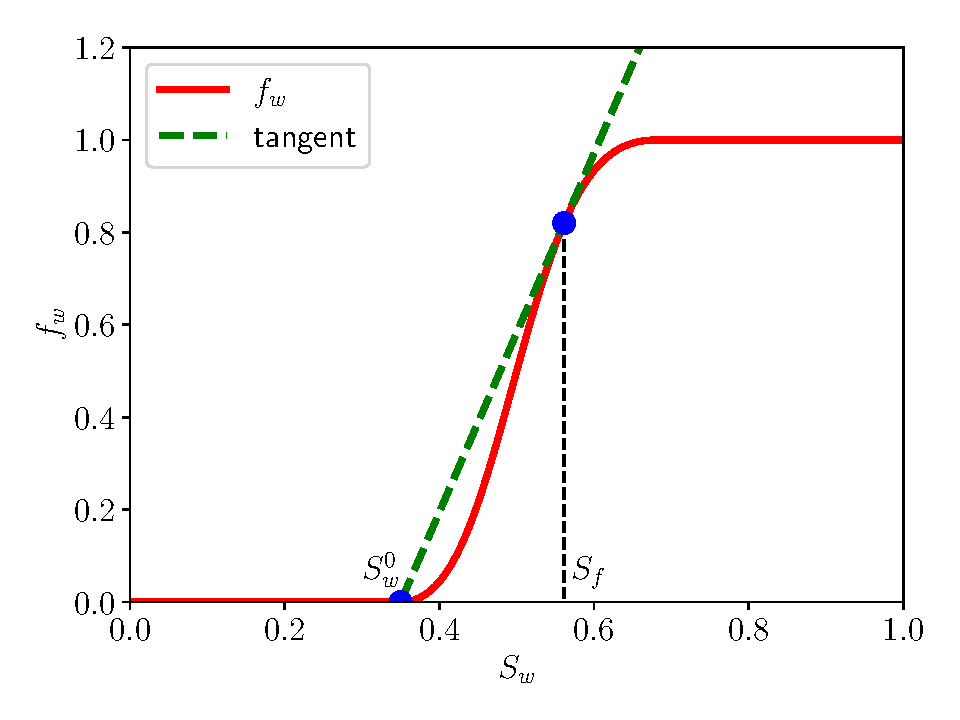
\includegraphics[width=0.7\linewidth]{img/FwCurveTangent}
	\caption{Точка соприкосновения кривой $f_w(S_w)$ и касательной проведенной из значения водоносыщенности перед фронтом ($S_w^0$) определяет водонасыщенность на фронте $S_f$}
	\label{fig:FwCurveTangent}
\end{figure}

Положение фронта в момент времени $t$ задается соотношением $x_f=q_{inj}\cdot f'(S_f)t /\phi$. Момент времени прорыва фронта в правую точку (когда фронт дойдет до точки $x=L$) определяется соотношением
$  t_{bf}=\phi L / (q_{inj} \,f'(S_f)).$


В частном случае, когда $S_w^0=S_w^{cr}$ и $n_w=n_o=2$, тогда $\overline{S}_w^0=0$, $f(\overline{S}_w^0)=0$ и
значение насыщенности на фронте находится аналитически в виде
\begin{equation}\label{eq:star:exact_sw}
  \overline{S}_f=\sqrt{\frac{k_{ro}^0/\mu_o}{k_{rw}^0/\mu_w+k_{ro}^0/\mu_o}}=\frac{1}{\sqrt{1+k_{rw}^0 \mu_o/ (\mu_w k_{ro}^0)}}.
\end{equation}
\bibliography{bibbase_local.bib}
\bibliographystyle{plain}

\end{document}
